
\section{Methodology}


\subsection{Approach}
This study adopts a quantitative and experimental approach to investigate the predictive relationship between yield curve dynamics and U.S. recessionary periods. The methodology is grounded in empirical modeling and computational experimentation, aiming to quantify the extent to which various term spreads and machine learning models can accurately forecast recessions.

The quantitative aspect is reflected in the use of structured time-series data and statistical indicators derived from Treasury yields, processed to generate explanatory features. The experimental component involves the systematic development, training, and evaluation of multiple predictive models under controlled conditions. These include traditional econometric models and modern machine learning classifiers, all tested on consistent datasets with standardized performance metrics. This dual approach ensures both the analytical rigor of hypothesis-driven modeling and the adaptability of data-driven experimentation.

\subsection{Data Collection}

This study utilizes secondary quantitative data obtained from publicly available economic datasets. The primary source of financial indicators is the Federal Reserve Bank of St. Louis (FRED), from which three daily time series were extracted: the 10-Year Treasury Constant Maturity Rate (GS10), the 2-Year Treasury Constant Maturity Rate (DGS2), and the 3-Month Treasury Bill Rate (DGS3MO). These yield series were selected due to their widespread use in macro-financial research and their theoretical linkage to expectations about future economic activity.

To identify recessionary periods for labeling, the study uses official dates provided by the \textcite{NBERRecession}. 


\subsection{Tools and Techniques}

Computational analysis for this research was conducted using Python3 within a Jupyter Notebook environment.

\begin{comment}
Key libraries used include:
\begin{itemize}
    \item \textbf{pandas} and \textbf{NumPy} for data manipulation and numerical computations;
    \item \textbf{scikit-learn} for classical machine learning models (e.g., Logistic Regression, Random Forest) and preprocessing utilities (e.g., SMOTE, train-test split);
    \item \textbf{xgboost} for gradient boosting classifiers;
    \item \textbf{imbalanced-learn} for handling class imbalance using ensemble methods and synthetic oversampling;
    \item \textbf{TensorFlow} and \textbf{Keras} for building, training, and tuning Long Short-Term Memory (LSTM) networks.
\end{itemize}
\end{comment}


\subsection{Data Analysis}

Initial preprocessing of the time-series data involved using forward-fill to handle missing values. This technique was chosen to maintain temporal continuity without introducing artificial volatility or structural breaks.
Subsequently, two features were engineered from the processed data: the 10-year minus 2-year Treasury spread (GS10--DGS2) and the 10-year minus 3-month Treasury spread (GS10--DGS3MO). 
A binary target variable was constructed based on the NBER-designated recession dates, labeling each daily observation as either within (1) or outside (0) a recession period. 
Following the creation of these three features, the dataset was further resampled into three distinct time frequencies: daily, weekly, and monthly. This would allow for the evaluation of model performance under varying levels of temporal aggregation and data granularity.  
The final feature engineered dataset spans 01-Jan-1982 to 18-Jul-2025%\hldefault{18-Jul-2025} 
and includes both recession and non-recession periods, facilitating robust training and evaluation of predictive models under realistic, imbalanced class distributions. \\

%\vspace{-9pt}

\begin{figure}[htbp]
    %\centering
    \raggedright
    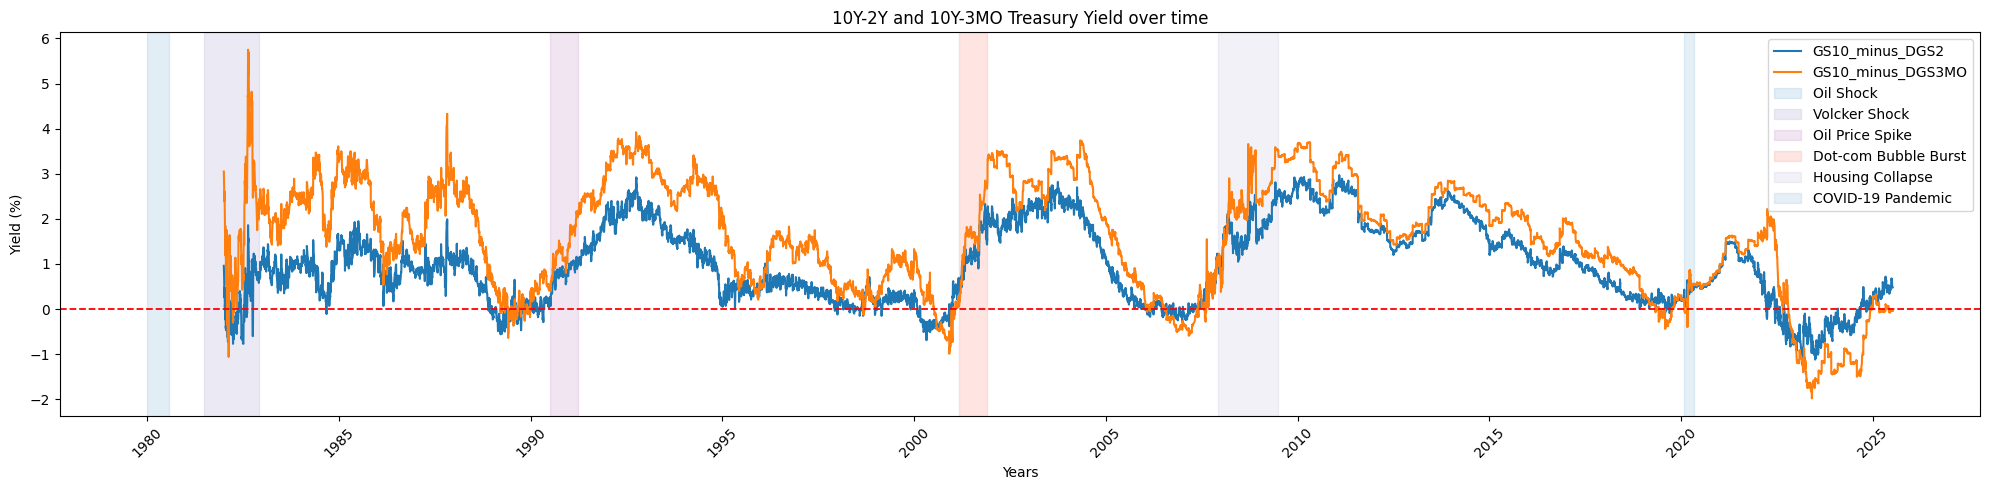
\includegraphics[
        width=\textwidth-24pt, 
        height=\textheight,%-24pt, 
        keepaspectratio
        ]
        {Steps/Plots/10Y-2Y and 10Y-3MO Treasury Yield over time.png}
    \caption{10Y-2Y and 10Y-3MO U.S. Treasury Yield Spreads Over Time. %Inversions (when the spread falls below zero) are often viewed as potential indicators of upcoming economic recessions.
    }
    \label{fig:yield-spreads}
\end{figure}

